\documentclass[11pt,a4paper]{article}%
\usepackage{amsmath,amsbsy,amssymb,amsfonts}
\usepackage{bm}
\usepackage{mathrsfs}
%\usepackage[colorlinks,unicode, bookmarksnumbered=true]{hyperref}
\usepackage{natbib}
\usepackage{graphicx}
\usepackage{array}
\usepackage{listings}
\usepackage{indentfirst}
\usepackage[amsmath,thmmarks,thref]{ntheorem}
\usepackage{stmaryrd}
\usepackage{url}
\usepackage{lscape}
\usepackage{tabularx}
\usepackage{longtable}
\usepackage{fancyhdr}
\usepackage{fancybox}
\usepackage{titlesec}
\usepackage{multirow}
\usepackage{booktabs}	
\usepackage{enumerate}
\usepackage{cases}
\usepackage{pstricks-add}
\usepackage{float}
\usepackage{subfigure}   %多图加小标题
\usepackage{hyperref}  % 引用超链接
\usepackage{booktabs} % 表格线
\usepackage{multirow}  % 表格内部合并
\usepackage{ulem} %划掉字符
\usepackage{caption}

\usepackage{threeparttable}



\pagestyle{fancy}
\setlength\textheight{230mm}
\setlength\textwidth{152mm}
\setlength\topmargin{-1mm}
\setlength\hoffset{-15mm}
\lhead{}
\chead{}
\rhead{}
\fancyfoot[C]{\hskip 30mm --- \thepage \ ---}
\renewcommand{\headrulewidth}{0pt}
\renewcommand{\headsep}{5pt}
\renewcommand{\footskip}{40pt}

\newcommand{\PreserveBackslash}[1]{\let\temp=\\#1\let\\=\temp}
\newcolumntype{C}[1]{>{\PreserveBackslash\centering}p{#1}}
\newcolumntype{R}[1]{>{\PreserveBackslash\raggedleft}p{#1}}
\newcolumntype{L}[1]{>{\PreserveBackslash\raggedright}p{#1}}

%===================== 重定义字体、字号命令 =============================%
%\iffalse
\newcommand{\CJKsong}[1]{{\CJKfamily{song}#1}}
\newcommand{\CJKkai}[1]{{\CJKfamily{kai}#1}}
\newcommand{\CJKhei}[1]{{\CJKfamily{hei}#1}}
\newcommand{\CJKfxk}[1]{{\CJKfamily{you}#1}}
\newcommand{\zhengwenziti}{song}
%
\newcommand{\song}{\CJKfamily{song}}
\newcommand{\fangsong}{\CJKfamily{fs}}
\newcommand{\kai}{\CJKfamily{kai}}
\newcommand{\hei}{\CJKfamily{hei}}
\newcommand{\lishu}{\CJKfamily{li}}
\newcommand{\fxk}{\CJKfamily{you}}
%\fi
%
%
\iffalse
\newcommand{\CJKsong}[1]{{\CJKfamily{gbsn}#1}}
\newcommand{\CJKkai}[1]{{\CJKfamily{gkai}#1}}
\newcommand{\CJKhei}[1]{{\CJKfamily{gbsn}#1}}
\newcommand{\CJKfxk}[1]{{\CJKfamily{gkai}#1}}
\newcommand{\zhengwenziti}{gbsn}
%
\newcommand{\song}{\CJKfamily{gbsn}}
\newcommand{\kai}{\CJKfamily{gkai}}
\newcommand{\hei}{\CJKfamily{gbsn}}
\newcommand{\songhei}{\CJKfamily{gbsn}}
\newcommand{\fxk}{\CJKfamily{gkai}}
\fi

\newcommand{\chuhao}{\fontsize{42pt}{\baselineskip}\selectfont}
\newcommand{\xiaochu}{\fontsize{36pt}{\baselineskip}\selectfont}
\newcommand{\yihao}{\fontsize{28pt}{\baselineskip}\selectfont}
\newcommand{\erhao}{\fontsize{21pt}{\baselineskip}\selectfont}
\newcommand{\xiaoerhao}{\fontsize{18pt}{\baselineskip}\selectfont}
\newcommand{\sanhao}{\fontsize{15.75pt}{\baselineskip}\selectfont}
\newcommand{\xiaosan}{\fontsize{15.1pt}{\baselineskip}\selectfont}
\newcommand{\sihao}{\fontsize{14pt}{\baselineskip}\selectfont}
\newcommand{\xiaosi}{\fontsize{12pt}{\baselineskip}\selectfont}
\newcommand{\wuhao}{\fontsize{10.5pt}{\baselineskip}\selectfont}
\newcommand{\xiaowuhao}{\fontsize{9pt}{\baselineskip}\selectfont}
\newcommand{\liuhao}{\fontsize{7.875pt}{\baselineskip}\selectfont}
\newcommand{\qihao}{\fontsize{5.25pt}{\baselineskip}\selectfont}

\newcommand{\institution}{}
\newcommand{\numberID}{}
\newcommand{\cardID}{}
\newcommand{\namestudent}{}
\newcommand{\namesupervisor}{}
\newcommand{\thestitlelineone}{}
\newcommand{\thestitlelinetwo}{}
\newcommand{\thestitlelinethree}{}
\newcommand{\discipline}{}
\newcommand{\myyear}{}
\newcommand{\mymonth}{}
\newcommand{\myday}{}
\newcommand{\researchtopic}{}

\iffalse
\newtheorem{scheme}{Scheme}
\newtheorem{theorem}{Theorem}[section]
\newtheorem{lemma}[theorem]{Lemma}
\newtheorem{corollary}[theorem]{Corollary}
\newtheorem{definition}{Definition}[section]
\newtheorem{algorithm}{Algorithm}
\newtheorem{assumption}{Assumption}[section]
\newtheorem{remark}{Remark}[section]
%\newdefinition{remark}{Remark}[section]
%\newdefinition{example}{Example}[section]
\newenvironment{proof}[1][Proof]{\noindent\textbf{#1. }}{\hfill $\Box$}
\fi

\def
\theequation{\thesection.\arabic{equation}}
%\numberwithin{equation}{section}


\titleformat{\section}{\xiaosi\bfseries}{\thesection .}{.3em}{}

% please place your own definitions here and don't use \def but
% \newcommand{}{}

\def
\theequation{\thesection.\arabic{equation}}
\numberwithin{equation}{section}
\newcommand*{\abs}[1]{\lvert#1\rvert}
\newcommand*{\Abs}[1]{\big\lvert#1\big\rvert}
\newcommand*{\ABS}[1]{\Big\lvert#1\Big\rvert}
%\newcommand*{\norm}[1]{\left\lVert #1 \right\rVert}
\newcommand*{\norm}[1]{\lVert #1 \rVert}
\newcommand*{\Norm}[1]{\big\lVert #1 \big\rVert}
\newcommand*{\NOrm}[1]{\Big\lVert #1 \Big\rVert}
\newcommand*{\NORM}[1]{\left\lVert #1 \right\rVert}
\newcommand*{\tnorm}[1]{\interleave#1\interleave}
\newcommand*{\jump}[1]{\llbracket #1\rrbracket}
%\newcommand*{\jump}[1]{\lBrack #1\rBrack}
\newcommand*{\Jump}[1]{\left\llbracket #1\right\rrbracket}
\newcommand*{\JUMP}[1]{\Big\llBracket #1 \Big\rrBracket}
\def\sech{\mathrm{sech}}
\def\mathi{\mathrm{i}}
%\newcommand\mathd{\mathrm{d}}
\newcommand\mathd{d}
\newcommand\bsm{\boldsymbol}
%\def\mathds{\mathrm{~d}}
%\def\mathdx{\mathrm{~d\bf{x}}}
\def\mathds{\,ds}
\def\mathdx{\,d{\bm x}}

\usepackage{CJKutf8,CJKnumb}%,CJKulem}
\AtBeginDocument{\begin{CJK}{UTF8}{song}}
	\AtEndDocument{\clearpage \end{CJK}}

\setlength{\parindent}{2em}
\linespread{1.3}

\begin{document}
	
\renewcommand\figurename{图}
\renewcommand\tablename{表}
\renewcommand\refname{参考文献}

\newtheorem{scheme}{格式}
\newtheorem{theorem}{定理}[section]
\newtheorem{lemma}{引理}[section]
\newtheorem{corollary}[theorem]{推论}
\newtheorem{definition}{定义}[section]
\newtheorem{algorithm}{算法}
\newtheorem{assumption}{假设}[section]
\newtheorem{remark}{注}[section]
%\newdefinition{remark}{Remark}[section]
\newtheorem{example}{例}[section]
\newenvironment{proof}[1][证明]{\noindent\textbf{#1. }}{\hfill $\Box$}
	
	
	
\renewcommand{\institution}{学院名称} % 数学与统计学院
\renewcommand{\numberID}{}
\renewcommand{\cardID}{1234567890}
\renewcommand{\namestudent}{张三}
\renewcommand{\namesupervisor}{李四~教授}
\renewcommand{\thestitlelineone}{博士论文选题名称}
\renewcommand{\thestitlelinetwo}{选题名称第二行} % 如果只有一行,可在content/cover中 注释掉 \thestitlelinetwo
\renewcommand{\discipline}{专业}
\renewcommand{\myyear}{2022}
\renewcommand{\mymonth}{6}
\renewcommand{\myday}{6}

\renewcommand{\em}{\it} % 期刊名去掉下划线

% page 1 2
\begin{center}
\raisebox{-18mm}{
\includegraphics[scale=0.33]{xjtu/xjtu1}} \hskip 44mm
\begin{tabular}{|C{22mm}|C{34mm}|}
	\hline
	\parbox[c][8.2mm][c]{0pt}{}{\kai\bf\xiaosi 学\hspace*{7mm} 院} & {\kai\bf\xiaosi\institution} \\
	\hline
	\parbox[c][8.2mm][c]{0pt}{}{\kai\bf\xiaosi 编\hspace*{7mm} 号} & {\kai\bf\xiaosi\numberID} \\
	\hline
	\end{tabular}\\
\vspace{8mm}
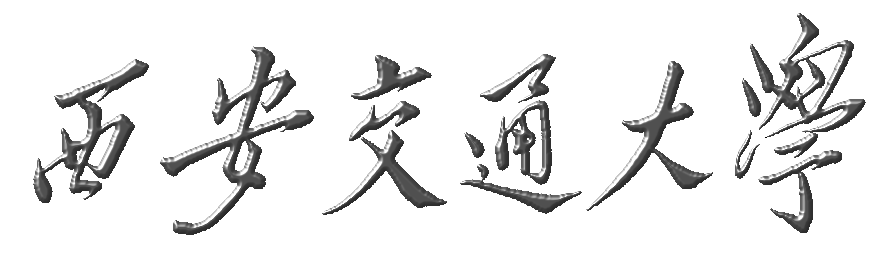
\includegraphics[scale=0.31]{xjtu/xjtu2}
\vspace{3mm}

{\song\xiaochu\bf
博士研究生\\[6mm]
中期进展报告}
\vspace{35mm}

{\large\sanhao%\renewcommand{\arraystretch}{0.9}
\renewcommand\arraystretch{1.32}
\begin{tabular}{lc}
\makebox[26mm][s]{\kai\bf\xiaosan 学    号:}   & \underline{\makebox[16em][c]{\xiaosan\kai\cardID}}\\
\makebox[26mm][s]{\kai\bf\xiaosan 研 究 生:}  & \underline{\makebox[16em][c]{ \xiaosan\kai\namestudent}}\\
\makebox[26mm][s]{\kai\bf\xiaosan 导   师:}   & \underline{\makebox[16em][c]{\xiaosan\kai\namesupervisor}}\\
\makebox[26mm][s]{\kai\bf\xiaosan 论 文 题 目:}& \underline{\makebox[16em][c]{\xiaosan\kai\thestitlelineone}}\\
                                               & \underline{\makebox[16em][c]{\xiaosan\kai\thestitlelinetwo}}\\
%                                           & \underline{\makebox[16em][c]{\xiaosan\kai\thestitlelinethree}}\\
\makebox[26mm][s]{\kai\bf\xiaosan 学    科:}   & \underline{\makebox[16em][c]{\xiaosan\kai\discipline}}\\
\makebox[26mm][s]{\kai\bf\xiaosan 填 写 时 间:}& \underline{\makebox[16em][c]{ \myyear ~年 \mymonth ~月 \myday ~日}}
\end{tabular}
}\\
\vspace{10mm}
{\kai\xiaosan 西安交通大学研究生院制}
\end{center}
\thispagestyle{empty}


\newpage
\vspace*{-7mm}
\begin{center}
\hei\xiaosan 填  写  说  明 \\
\vspace{15mm}
\begin{minipage}{13.6cm}
{%\linespread{1.5}
\song\sihao
\hspace{1.6em} 一、博士研究生中期进展报告必须采用 A4 纸双面打印,左侧装订成册,各栏空格不够时,请自行加页。格式可在研究生院主页下载。\vspace*{2mm}
\par \linespread{1.5} \hspace{1.6em} 二、中期进展报告正文部分字数为 8000-10000 字。\vspace*{2mm}
\par \linespread{1.5} \hspace{1.6em} 三、博士研究生中期进展报告通过后,\vspace*{2mm} 本报告由学院存档,并作为必修环节,登入成绩。
}
\end{minipage}
\end{center}

\thispagestyle{empty}

% main.tex
\newpage
\setcounter{page}{1}
\fancypage{%
\setlength{\fboxsep}{8pt}%
\setlength{\fboxrule}{0.8pt}%
\setlength{\shadowsize}{0pt}%
\shadowbox}{}
\setcounter{page}{1}

\begin{table}
\vspace{-3mm}
\arrayrulewidth=0.8pt
\hspace{-4mm}
\begin{tabular}{C{33mm}C{117mm}}
\hline
\parbox[c][15mm][c]{0pt}{}{\song\xiaosi\bf 研究题目} \hspace{2mm} \vline &   {\xiaosi\kai\researchtopic} 博士论文选题题目 \\
	\hline
\end{tabular}
\end{table}

\noindent{\xiaosi\song\bf 一、研究内容简介(300~500字)}
% Part 1
% 一、研究内容简介(300~500字)
\par
博士论文研究摘要






\newpage
\noindent{\xiaosi\song\bf 二、研究工作进展(包括已经完成的主要工作内容以及已经取得的成绩。本部分为主体部分,请详细叙述。)}
% part2
%二、研究工作进展(包括已经完成的主要工作内容以及已经取得的成绩。本部分为主体部分,请详细叙述。)

\section*{目前已经取得的研究工作成绩(一篇一作、一篇二作发表,一篇一作在审)}
\begin{description}
  \item[1] \textbf{K. He}, X. Zhang, S. Ren, and J. Sun, “Deep residual learning for image recognition,” in Proceedings of the IEEE Conference on Computer Vision and Pattern Recognition (CVPR), June 2016.
  \item[2] S. Ren, \textbf{K. He}, R. Girshick, and J. Sun, “Faster r-cnn: Towards real-time object detection with region proposal networks,” Advances in neural information processing systems,
vol. 28, 2015.
  \item[3] \textbf{K. He}, X. Chen, S. Xie, Y. Li, P. Doll´ar, and R. Girshick, “Masked autoencoders are scalable vision learners,” Submitted to the Proceedings of the IEEE/CVF Conference on Computer Vision and Pattern Recognition (CVPR), 2022
\end{description}

\section*{已完成的主要工作内容详细介绍}

\section{研究内容简介}
研究内容简介部分


\section{第一项研究工作题目}

\subsection{研究背景}
研究背景,引用\cite{ResNet}


\subsection{相关研究工作}

\subsubsection{相关研究工作1}
相关研究工作1

\begin{figure}[H]
  \centering
  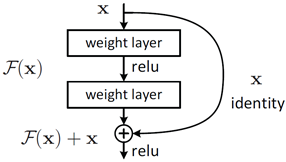
\includegraphics[scale = 0.8]{pictures/1.jpg}
  \caption{\small Residual Block.}
  \label{Architecture}
\end{figure}


\subsubsection{相关研究工作2}
相关研究工作2


\subsection{提出算法模型}
提出算法

\subsection{实验结果与分析}
实验结果与分析

\subsection{结论}
结论部分
  % 第一项研究工作
\section{第二项研究工作题目}

\subsection{研究背景}
研究背景,引用\cite{FasterRCNN}、引用\cite{MAE}


\subsection{相关研究工作}

\subsubsection{相关研究工作1}
相关研究工作1


\subsubsection{相关研究工作2}
相关研究工作2


\subsection{提出算法模型}
提出算法

\subsection{实验结果与分析}
实验结果与分析

\subsection{结论}
结论部分
  % 第二项研究工作
%\input{part23}  % 第三项研究工作
%\input{part23}

\bibliographystyle{IEEEtran}
\normalem % 去掉期刊名下划线
\bibliography{articles}

%\bibliographystyle{abbrv}
%\bibliography{articles}





\newpage
\noindent{\xiaosi\song\bf 三、下一步的工作计划}
% part3
% 三、下一步的工作计划

\begin{enumerate}
    \item 研究计划一。
    \item 研究计划二。
\end{enumerate}


\newpage
\noindent{\xiaosi\song\bf 四、导师评语}\\
% part4
% 四、导师评语
\par 导师评语。


\vfill
\hskip 4cm  {\xiaosi\song\bf 签名:\hskip 4cm 日期:\qquad 年 \quad 月 \quad 日}

%\bibliographystyle{unsrt}
\bibliographystyle{abbrv}
%\bibliographystyle{IEEEtran}
%\bibliographystyle{model1-num-names}
%\bibliography{Multi_bibfile,Phase_Field_bibfile_PFC,Phase_Field_bibfile}
%\bibliography{articles}

\end{document}
